\documentclass[10pt]{beamer}

\usepackage{gensymb}
\usepackage{graphicx}
\usepackage{wrapfig}
\usepackage{attrib}
\usepackage{textpos}

\usetheme{Dresden}
\usecolortheme{dove}
\usenavigationsymbolstemplate{}
\title{Research?}
\author{Pieter Brederode, Timo Koppenberg, \\ Jelco Bodewes, Anton Golov}
\institute{B3OMI}


\begin{document}

\begin{frame}
    \maketitle
\end{frame}


\section{Introduction}
\begin{frame}{Overview}
    \begin{itemize}
        \item We did research!
        \item That's it, really.
    \end{itemize}
\end{frame}

\section{Results}

\begin{frame}{Results}
    \begin{itemize}
        \item 117 different setups.
        \item 19 runs, for a total of 2223 cases.
    \end{itemize}
\end{frame}

\begin{frame}{Amount of entries}
	\begin{figure}
	  \centering
	    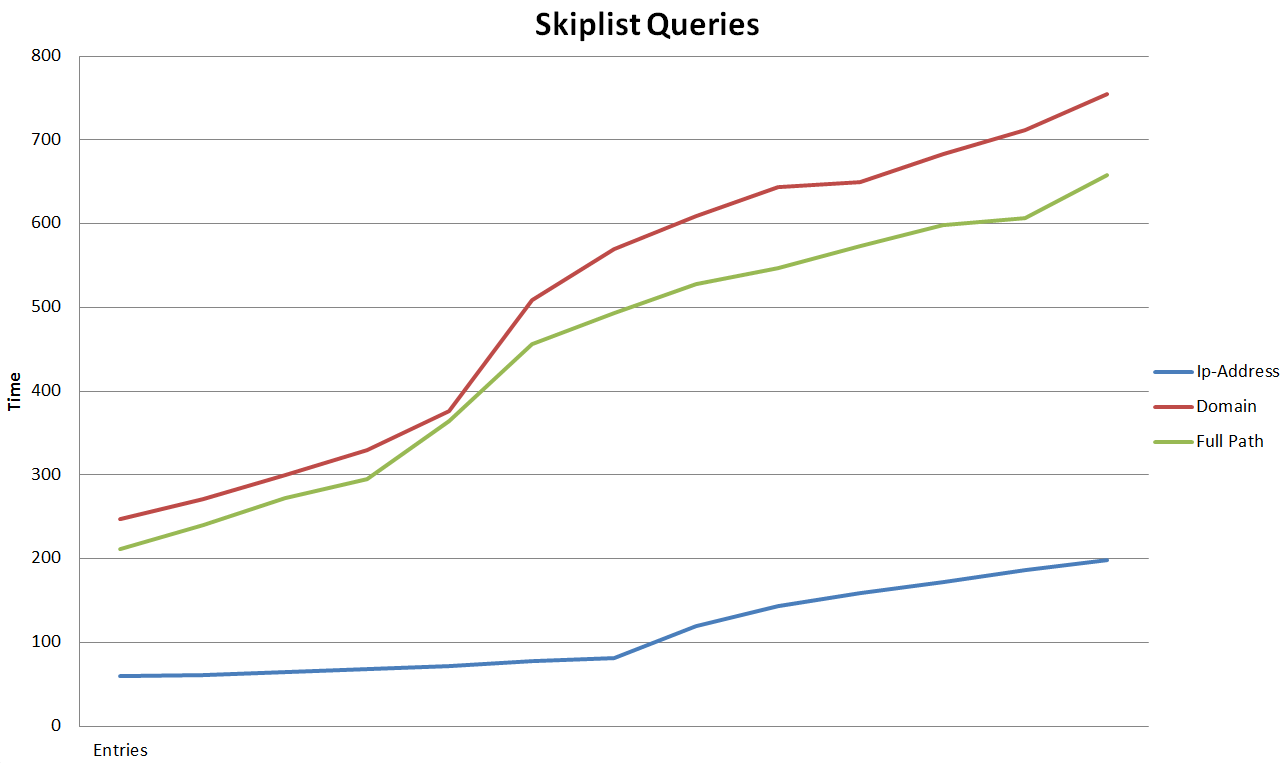
\includegraphics[width=0.95\textwidth]{SkiplistQuery}
	  \caption{The average amount of time for each query operation, plotted against the total number of entries.}
	\end{figure}
\end{frame}

\begin{frame}{Amount of entries}
    \begin{itemize}
        \item There is a positive correlation between the amount of entries and the average speed of all structures.
        \item This is true for both insert and query average speed.
        \item Not always true for average memory usage.
    \end{itemize}       
\end{frame}

\begin{frame}{Amount of entries}
    \begin{itemize}
        \item Average memory usage for BST is constant.
        \item Average memory usage for Hashmap has a positive correlation with the amount of entries.
        \item Average memory usage for Skiplist has a negative correlation with the amount of entries.
    \end{itemize}
\end{frame}

\begin{frame}{Amount of entries}
	\begin{figure}
	  \centering
	    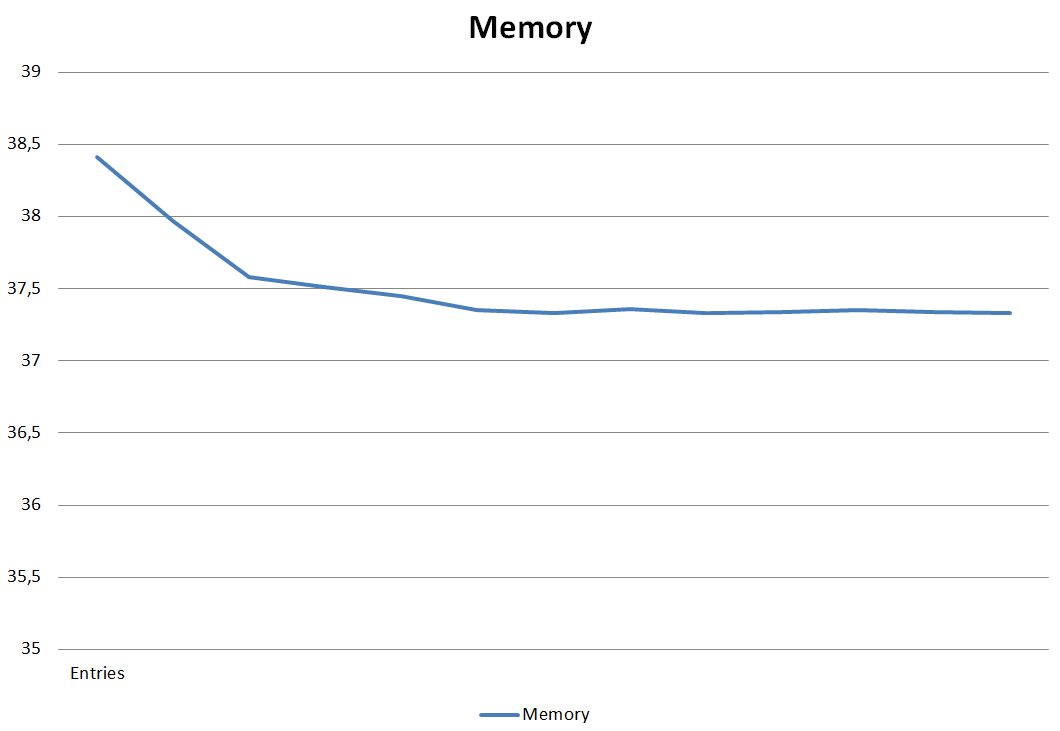
\includegraphics[width=0.95\textwidth]{SkiplistMemory}
	  \caption{The average amount of time for each query operation, plotted against the total number of entries.}
	\end{figure}
\end{frame}

\begin{frame}{Binary search tree}
    \begin{itemize}
        \item For Ip-Adresses: Significantly faster insertions than both other structures for low amount of entries.
        \item Scales badly compared to the other structures.
        \item Other keys: Always slower than Hashmap.
    \end{itemize}       
\end{frame}

\begin{frame}{Hashmap}
    \begin{itemize}
        \item Significantly faster query speed in all situations compared to other structures.
        \item Faster insert speed as well in most situations.
        \item Highest amount of memory usage in all cases.
    \end{itemize}       
\end{frame}

\begin{frame}{Skiplist}
    \begin{itemize}
        \item In no tested situations the fasted structure.
        \item Similar performance to BST for large amount of entries.
        \item Always the lowest memory usage, average memory usage goes down with more entries.
    \end{itemize}       
\end{frame}

\section{Conclusions}

\begin{frame}{Conclusions}
    \begin{itemize}
        \item Hashmap usually the best option.
        \item Binary search tree better for small amounts of simple keys.
        \item Skiplist useful for low memory usage.
    \end{itemize}
\end{frame}

\end{document}
